\documentclass{article}

% if you need to pass options to natbib, use, e.g.:
% \PassOptionsToPackage{numbers, compress}{natbib}
% before loading nips_2017
%
% to avoid loading the natbib package, add option nonatbib:
% \usepackage[nonatbib]{nips_2017}

\usepackage{nips_2017}
\usepackage{dsfont}
% to compile a camera-ready version, add the [final] option, e.g.:
% \usepackage[final]{nips_2017}

\usepackage[utf8]{inputenc} % allow utf-8 input
\usepackage[T1]{fontenc}    % use 8-bit T1 fonts
\usepackage{hyperref}       % hyperlinks
\usepackage{url}            % simple URL typesetting
\usepackage{booktabs}       % professional-quality tables
\usepackage{amsfonts}       % blackboard math symbols
\usepackage{nicefrac}       % compact symbols for 1/2, etc.
\usepackage{microtype}      % microtypography

\usepackage{graphicx} % more modern
%\usepackage{epsfig} % less modern
%\usepackage{subfig} 
\usepackage{fancyvrb}

\usepackage{caption}
\usepackage{subcaption}

\fvset{fontsize=\footnotesize}


\usepackage{multirow}
\usepackage{array}

\usepackage{amssymb}
\usepackage{listings}
\usepackage{wrapfig}
\usepackage{tabularx}


\usepackage{verbatim}
 \usepackage{booktabs}
 % For algorithms
\usepackage{algorithm}
\usepackage{algorithmic}
\usepackage{tikz}
\usetikzlibrary{fit}
\usetikzlibrary{arrows.meta}
\usetikzlibrary{positioning}
\usetikzlibrary{decorations.text}
\usetikzlibrary{decorations.pathmorphing}

% As of 2011, we use the hyperref package to produce hyperlinks in the
% resulting PDF.  If this breaks your system, please commend out the
% following usepackage line and replace \usepackage{icml2016} with
% \usepackage[nohyperref]{icml2016} above.
\usepackage{amsmath}
\usepackage{hyperref}
\DeclareMathOperator*{\argmin}{arg\,min} % thin space, limits underneath in displays
\DeclareMathOperator{\argmin}{argmin} % no space, limits underneath in displays
\DeclareMathOperator*{\argmax}{arg\,max} % thin space, limits underneath in displays
\DeclareMathOperator{\argmax}{argmax} % no space, limits underneath in displays

\newcommand{\expect}{\mathds{E}} %{{\rm I\kern-.3em E}}
\newcommand{\probability}{\mathds{P}} %{{\rm I\kern-.3em P}}

\newcommand{\remark}[1]{\textcolor{red}{[#1]}}


\title{Inferring Graphics Programs from Images}

% The \author macro works with any number of authors. There are two
% commands used to separate the names and addresses of multiple
% authors: \And and \AND.
%
% Using \And between authors leaves it to LaTeX to determine where to
% break the lines. Using \AND forces a line break at that point. So,
% if LaTeX puts 3 of 4 authors names on the first line, and the last
% on the second line, try using \AND instead of \And before the third
% author name.

\author{
  David S.~Hippocampus\thanks{Use footnote for providing further
    information about author (webpage, alternative
    address)---\emph{not} for acknowledging funding agencies.} \\
  Department of Computer Science\\
  Cranberry-Lemon University\\
  Pittsburgh, PA 15213 \\
  \texttt{hippo@cs.cranberry-lemon.edu} \\
  %% examples of more authors
  %% \And
  %% Coauthor \\
  %% Affiliation \\
  %% Address \\
  %% \texttt{email} \\
  %% \AND
  %% Coauthor \\
  %% Affiliation \\
  %% Address \\
  %% \texttt{email} \\
  %% \And
  %% Coauthor \\
  %% Affiliation \\
  %% Address \\
  %% \texttt{email} \\
  %% \And
  %% Coauthor \\
  %% Affiliation \\
  %% Address \\
  %% \texttt{email} \\
}

\begin{document}
% \nipsfinalcopy is no longer used

\maketitle

\begin{abstract}
\end{abstract}

\section{Introduction}

 How could an agent go from noisy, high-dimensional perceptual input
 to a symbolic, abstract object, like a computer program?  Here we
 consider this problem within a graphics program synthesis domain.  We
 develop an approach for converting natural images, such as hand
 drawings, into executable source code for drawing the original image.
 The graphics programs in our domain draw simple figures like those found in
 machine learning papers (see Fig.\ref{firstPageExamples}).
 \remark{The use of `graphics programs / visual programs' in the paper
   title, title of this section, and the body of this section feels
   too broad. `Graphics program' could conjur a lot of different ideas
   (esp. 3D graphics); don't want to set the reader up to expect one
   thing and then be disappointed that what you've done isn't
   that. You bring up diagram-drawing later in the intro; I think it
   should be made clear sooner (and certainly mentioned explicitly in
   the abstract, when you get around to writing that).}

\newcommand{\exampleImageSize}{2cm}
\begin{figure}[h]
  \begin{minipage}[t]{0.7\linewidth}  
\begin{tabular}{llll}
  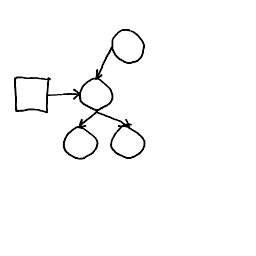
\includegraphics[width = \exampleImageSize]{figures/expert-60.png}&
  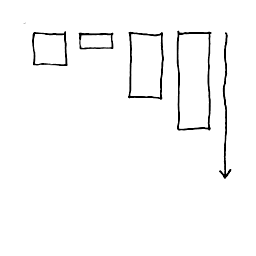
\includegraphics[width = \exampleImageSize]{figures/expert-5.png}&
    \includegraphics[width = \exampleImageSize]{figures/expert-17.png}&
    \includegraphics[width = \exampleImageSize]{figures/expert-58.png}\\
  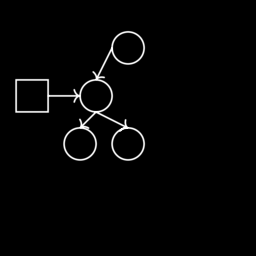
\includegraphics[width = \exampleImageSize]{figures/60.png}&
  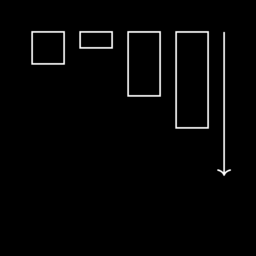
\includegraphics[width = \exampleImageSize]{figures/5.png}&
    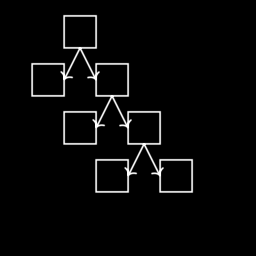
\includegraphics[width = \exampleImageSize]{figures/17.png}&
    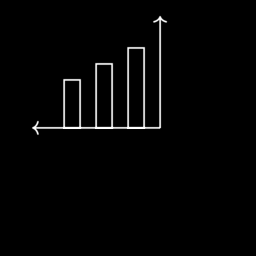
\includegraphics[width = \exampleImageSize]{figures/58.png}
\end{tabular}
\subcaption{}
  \end{minipage}%
  \begin{minipage}[t]{0.3\linewidth}
    \begin{tikzpicture}
      \node(picture) at (0,0) {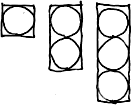
\includegraphics[width = 2cm]{figures/expert-31.png}};
      \draw[very thick,->] (picture.south)  -- (0,-2);
    \end{tikzpicture}\\
    \texttt{for} $0\leq i < 4$:\\
    \texttt{rectangle} $(-3i + 9,2i - 2, -3i + 11,6)$\\
    \texttt{for} $0\leq j < i$:\\
    \texttt{circle} $(3i-2,-2j+5)$\\
    \subcaption{}
  \end{minipage}
  \caption{(a): Model learns to convert hand drawings (top) into \LaTeX~(bottom). (b) Synthesizes high-level \emph{graphics program} from hand drawing.}\label{firstPageExamples}
  \end{figure}

High dimensional perceptual input may seem ill matched to the abstract
semantics of a programming language. But programs with constructs like
recursion or iteration produce a simpler \emph{execution trace} of
primitive actions; for our domain the primitive actions are drawing
commands. Our hypothesis is that the execution trace of the program is
better aligned with the perceptual input, and that the trace can act
as a kind of bridge between perception and programs. We test this
hypothesis by developing a model that learns to map from an image to
the execution trace of the graphics program that drew it.  With the
execution trace in hand, we can bring to bear techniques from the
program synthesis community to recover the latent graphics program.
This family of techniques, called \emph{constraint-based program synthesis}~\cite{solar2008program},
work by modeling a set of possible programs inside of a constraint solver,
like a SAT or SMT solver~\cite{de2008z3}.
These techniques excel at uncovering high-level symbolic structure,
but are not well equipped to deal with real-valued perceptual inputs.


We develop a hybrid architecture for inferring graphics programs.  Our
approach uses a deep neural network infer an execution trace from an
image; this network recovers primitive drawing operations such as
lines, circles, or arrows, along with their parameters. For added
robustness, we use the deep network as a proposal distribution for a
stochastic search over execution traces.  Finally, we use techniques
in the program synthesis community to recover the program from its
trace.  The program synthesizer discovers constructs like loops and
geometric operations like reflections and affine transformations.
\remark{This paragraph is all about making things a bit more specific,
  so you really need more specifics about program synth here.}

Each of these three components -- the deep network, the stochastic
search, the program synthesizer -- confers its own advantages. From
the deep network, we get a fast system that can recover plausible
execution traces in about a minute~\remark{A minute seems slow to me, for deep net inference. Are you talking about training time, here, or...?}. From the stochastic search we get
added robustness; essentially, the stochastic search can correct
mistakes made by the deep network's proposals.  From the program
synthesizer, we get abstraction: our system recovers coordinate
transformations, for loops, and subroutines, which are useful for
downstream tasks and can help correct some mistakes of the earlier stages.
\remark{I wonder if this would work even better as a bulleted list...}


\section{Related work}
attend infer repeat:~\cite{eslami1603attend}. Crucial distinction is
that they focus on learning the generative model jointly with the
inference network. Advantages of our system is that we learn symbolic
programs, and that we do it from hand sketches rather than synthetic
renderings.

ngpm:~\cite{ritchie2016neurally}. We build on the idea of a guide program, extending it to scenes composed of objects, and then show how to learn programs from the objects we discover.

Sketch-n-Sketch:~\cite{Hempel:2016:SSP:2984511.2984575}. Semiautomated synthesis presented in a nice user interface. Complementary to our work: you could pass a sketch to our system and then pass the program to sketch-n-sketch


Converting hand drawings into procedural models using deep networks:~\cite{huang2017shape,Nishida:2016:ISU:2897824.2925951}.



\section{Neural architecture for inferring drawing execution traces}

We developed a deep network architecture for efficiently inferring a
execution trace, $T$, from an image, $I$.  Our model constructs the
trace one drawing command at a time.  When predicting the next drawing
command, the network takes as input the target image $I$ as well as
the rendered output of previous drawing commands.  Intuitively, the
network looks at the image it wants to explain, as well as what it has
already drawn.  It then decides either to stop drawing or proposes
another drawing command to add to the execution trace; if it decides
to continue drawing, the predicted primitive is rendered to its
``canvas'' and the process repeats.

Figure~\ref{architecture} illustrates this architecture.  We first
pass a $256\times 256$ target image and a rendering of the trace so
far to a convolutional network -- these two inputs are represented as
separate channels for the convnet. Given the features extracted by the
convnet, a multilayer perceptron then predicts a distribution over the
next drawing command to add to the trace.  We predict the drawing
command token-by-token, and condition each token both on the image
features and on the previously generated tokens.  For example, the
network first decides to emit the \verb|circle| token conditioned on
the image features, then it emits the $x$ coordinate of the circle
conditioned on the image features and the \verb|circle| token, and
finally it predicts the $y$ coordinate of the circle conditioned on
the image features, the \verb|circle| token, and the $x$ coordinate.
\remark{There are some more details that are important to provide
  about this architecture, though possibly in an Appendix: the
  functional form(s) of the probability distributions over tokens, the
  network layer sizes, which MLPs share parameters, etc.}

\remark{Planning to move the description of SMC / beam search up here, too?}

The distribution over the next drawing command factorizes:
\begin{equation}
  \probability_\theta [t_1t_2\cdots t_K | I,T] = \prod_{k = 1}^K \probability_\theta [t_k | f_\theta(I,\text{render}(T)), \{t_j\}_{j = 1}^{k - 1}]
\end{equation}
where $t_1t_2\cdots t_K$ are the tokens in the drawing command, $I$ is
the target image, $T$ is an execution trace, $\theta$ are the
parameters of the neural network, and $f_\theta(\cdot,\cdot)$ is the
image feature extractor (convolutional network). The distribution over
execution traces factorizes as:
\begin{equation}
  \probability_\theta [T|I] = \prod_{n = 1}^{|T|} \probability_\theta [T_n | I,T_{1:(n-1)}]\times\probability_\theta [\verb|STOP| | I,T]\label{objective}
\end{equation}
where $|T|$ is the length of execution trace $T$, and the \verb|STOP|
token is emitted by the network to signal that the execution trace
explains the image.

We train the network by sampling execution traces $T$ and target
images $I$ for randomly generated scenes, and maximizing
(\ref{objective}) wrt $\theta$ by gradient ascent.
Training does not require backpropagation across the entire sequence of drawing commands:
drawing to the canvas `blocks' the gradients,
effectively offloading memory to an external visual store.
In a sense, this model is like an autoregressive variant of AIR~\cite{eslami1603attend} without attention.

\remark{I like that you make this connection, but it could be made more precisely. Specifically, (1) the architecture isn't \emph{really} recurrent (it uses no hidden state cells), so it'd be good to use a different term or drop this part of the point: (2) training of recurrent nets is also typically fully-supervised (Most RNNs lack latent variables per timestep)---if you're thinking about AIR specifically, maybe just say that, and (3) it's like an autogressive AIR \emph{without attention}.}
\remark{Something related to this that's also cool to point out: training this model doesn't require backpropagation across the entire sequence of drawing commands (drawing to the canvas `blocks' the gradients, effectively offloading memory to an external (visual) store, so in principle it might be scalable to much longer sequences.}

%% When we
%% have the generative model (the rendering function) and treat the trace
%% as fully observed, we need not solve an unsupervised or reinforcement
%% learning problem.
\tikzset{>=latex}
\begin{figure}
  \begin{tikzpicture}
  \node[draw,blue,ultra thick,anchor = west,inner sep=0pt,label=below:Target image: $I$](observation) at (0,-1) {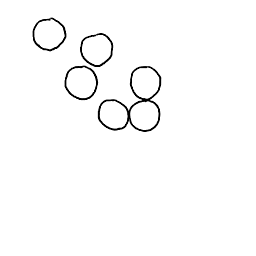
\includegraphics[width = 2cm]{figures/expert-18.png}};
  \node[draw,blue,thick,anchor = west,inner sep=0pt,minimum width = 2cm,minimum height = 2cm,label=below:Canvas: render$(T)$] (canvas) at (0,-4) {};
  \draw[lightgray,ultra thin,step = 0.125] ([xshift = 0.5,yshift = 0.5]canvas.south west) grid ([xshift = -0.5,yshift = -0.5]canvas.north east);
  % draw partial image on canvas
  \draw (0.5cm,-4cm) circle (0.1875cm);
  \draw (1.2cm,-4.3) circle (0.1875cm);
  \draw (0.85cm,-4.6) circle (0.1875cm);

  \node[draw,ultra thick,anchor = west,inner sep=0pt,minimum width = 2cm,minimum height = 3cm] (CNN) at (4.5,-2.5) {CNN};
  \node[inner sep = 0pt](tensorProduct) at ([xshift = -1.5cm]CNN.west) {$\bigotimes$};

  \node[rotate = -90,draw,ultra thick,inner sep=0pt,minimum width = 3cm,minimum height = 0.5cm] (features) at ([xshift = 1.5cm]CNN.east) {Image features};

  \node[draw,ultra thick,minimum size = 1cm](c1) at ([xshift = 1.5cm]features.north) {MLP};
  \node(l1) at ([yshift = -2cm]c1.south) {\verb|circle(|};
  \node[draw,ultra thick,minimum size = 1cm](c2) at ([xshift = 1cm]c1.east) {MLP};
  \draw[->,ultra thick,red] (c1.south) -- (l1.north);
  \node(l2) at ([yshift = -2cm]c2.south) {\verb|X=3,|};
  \draw[->,ultra thick,red] (c2.south) -- (l2.north);
  \node[draw,ultra thick,minimum size = 1cm](c3) at ([xshift = 1cm]c2.east) {MLP};
  \node(l3) at ([yshift = -2cm]c3.south) {\verb|Y=14)|};
  \draw[->,ultra thick,red] (c3.south) -- (l3.north);

  
  \draw[->,ultra thick] (features.north) -- (c1.west);
  \draw[->,ultra thick] (features.north) to[out = 45,in = 90] (c2.north);
  \draw[->,ultra thick] (features.north) to[out = 70,in = 90] (c3.north);
  \draw[->,ultra thick] ([xshift = 0.25cm]l1.north) -- (c2.west);
  \draw[->,ultra thick] ([xshift = 0.25cm]l1.north) -- (c3.west);
  \draw[->,ultra thick] ([xshift = 0.25cm]l2.north) -- ([yshift = -0.2cm]c3.west);

  \node(next)[draw,very thick,fit = (l1) (l2) (l3), dashed, label = below:{Next line of code}] {};

  \draw[-{>[scale = 1.5]},very thick,dashed] (next.west) -- ([yshift = -0.2cm]canvas.east) node [midway, below, sloped] (TextNode) {Renderer: \LaTeX};
  
  \draw[->,ultra thick] (canvas.east) -- (tensorProduct.south);%[yshift = -0.5cm]CNN.west);
  \draw[->,ultra thick] (observation.east) -- (tensorProduct.north);%([yshift = 0.5cm]CNN.west);
  \draw[->,ultra thick] (tensorProduct.east)  -- node[center,fill = white,rotate = 90] {{\tiny $256\times 256\times 2$}}  (CNN.west);
  \draw[->,ultra thick] (CNN.east) -- node[center,fill = white,rotate = 90] {{\tiny $16\times 16\times 10$}} (features.south);
%  \draw[]
  
%  \node at (canvas.x,canvas.y) {Canvas};
\end{tikzpicture}
\caption{Our neural architecture for inferring the execution trace of a graphics program from its output. \textcolor{blue}{Blue}: network inputs. Black: network operations. \textcolor{red}{Red}: samples from a multinomial. \texttt{Typewriter font}: network outputs. Renders snapped to a $16\times 16$ grid, illustrated in \textcolor{gray}{gray}.~\remark{Thoughts on improving this figure: (1) Convnet diagrams typically show the sequence of layers, if possible (space might not permit it here, but those thin arrows just aren't doing it for me). (2) Are the target image / canvas convolved down independently, or jointly (i.e. starting as a 2-channel image)? That's an important detail that's not clear with the current figure/explanation. (3) The three circles downstream from `Image Features' are supposed to be MLPs, I assume(?), but it took me a little while to parse that. Having some visual way of clearly separating network operations from data (color, perhaps) would go a long way.}}  \label{architecture}
\end{figure}
\begin{table}
\begin{tabular}{ll}\toprule
  \begin{tabular}{l}
    \verb|circle|$(x,y)$
  \end{tabular}& \begin{tabular}{l}
    Circle at $(x,y)$
    \end{tabular}\\
  \begin{tabular}{l}
    \verb|rectangle|$(x_1,y_1,x_2,y_2)$
  \end{tabular}&\begin{tabular}{l}
    Rectangle with corners at $(x_1,y_1)$ \& $(x_2,y_2)$
    \end{tabular}\\
  \begin{tabular}{l}
    \verb|LINE|$(x_1,y_1,x_2,y_2,$\\
    \hspace{1cm}$\text{arrow}\in\{0,1\},\text{dashed}\in\{0,1\})$
  \end{tabular}&\begin{tabular}{l}
    Line from $(x_1,y_1)$ to  $(x_2,y_2)$,\\\hspace{1cm}optionally with an arrow and/or dashed
    \end{tabular}\\
  \begin{tabular}{l}
    \verb|STOP|
  \end{tabular}&\begin{tabular}{l}
    Finishes execution trace inference
    \end{tabular}
\\  \bottomrule
\end{tabular}
\caption{The deep network in (\ref{architecture}) predicts drawing commands, shown above.}
\label{drawingCommandTable}
\end{table}



This network suffices to ``derender'' images like those shown in
Figure~\ref{trainingData}.  We can perform a beam search decoding to
recover what the network thinks is the most likely execution trace for
images like these. But, if the network makes a mistake (predicts an
incorrect line of code), it has no way of recovering from the error.
In order to derender an image with $n$ objects, it must correctly
predict $n$ drawing commands -- so its probability of success will
decrease exponentially in $n$, assuming it has any nonzero chance of
making a mistake.  For added robustness as $n$ becomes large, we treat
the neural network outputs as proposals for a SMC sampling scheme.
For the SMC sampler, we use pixel wise distance as a surrogate for a
likelihood function; see supplement. Figure~\ref{syntheticResults}
compares the neural network with SMC against the neural network by
itself or SMC by itself.  Only the combination of the two passes a
critical test of generalization: when trained on images with $\leq 8$
objects, it successfully parses scenes with many more objects than the
training data.
\begin{wrapfigure}{R}{0.5\textwidth}
  \begin{center}
    \begin{minipage}[t]{2.2cm}\fbox{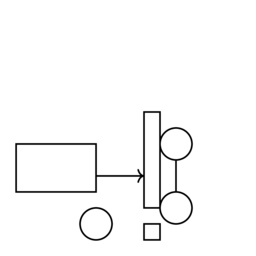
\includegraphics[width=2cm]{figures/randomScene-58-7.png}}\end{minipage}
    \begin{minipage}[t]{2.2cm}\fbox{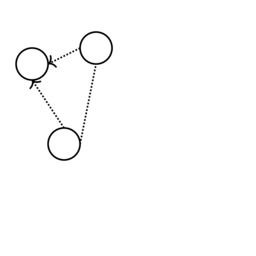
\includegraphics[width=2cm]{figures/randomScene-33-5.png}}\end{minipage}
    \begin{minipage}[t]{2.2cm}\fbox{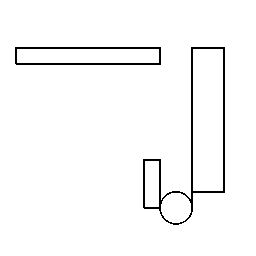
\includegraphics[width=2cm]{figures/randomScene-25-4.png}}\end{minipage}
%    \begin{minipage}[t]{2cm}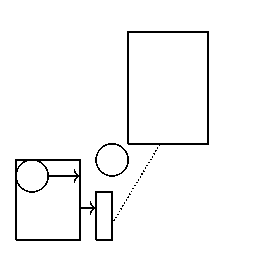
\includegraphics[width=2cm]{figures/randomScene-26-7.png}\end{minipage}
%    \begin{minipage}[t]{2cm}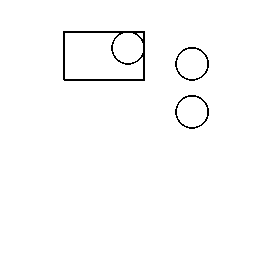
\includegraphics[width=2cm]{figures/randomScene-19-3.png}\end{minipage}
  \end{center}
  \caption{Network is trained to infer execution traces for figures like the three shown above.}\label{trainingData}
\end{wrapfigure}

\begin{figure}
  \begin{minipage}[t]{15cm}
    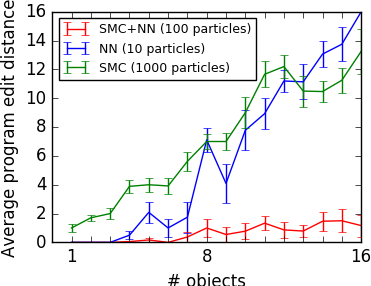
\includegraphics[width = 15cm]{figures/editDistance.png}
  \end{minipage}\\
  \begin{minipage}[t]{15cm}
    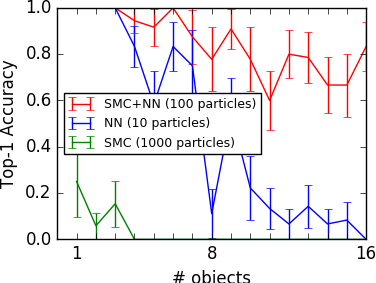
\includegraphics[width = 15cm]{figures/accuracy.png}
  \end{minipage}\\
  \begin{minipage}[t]{15cm}
    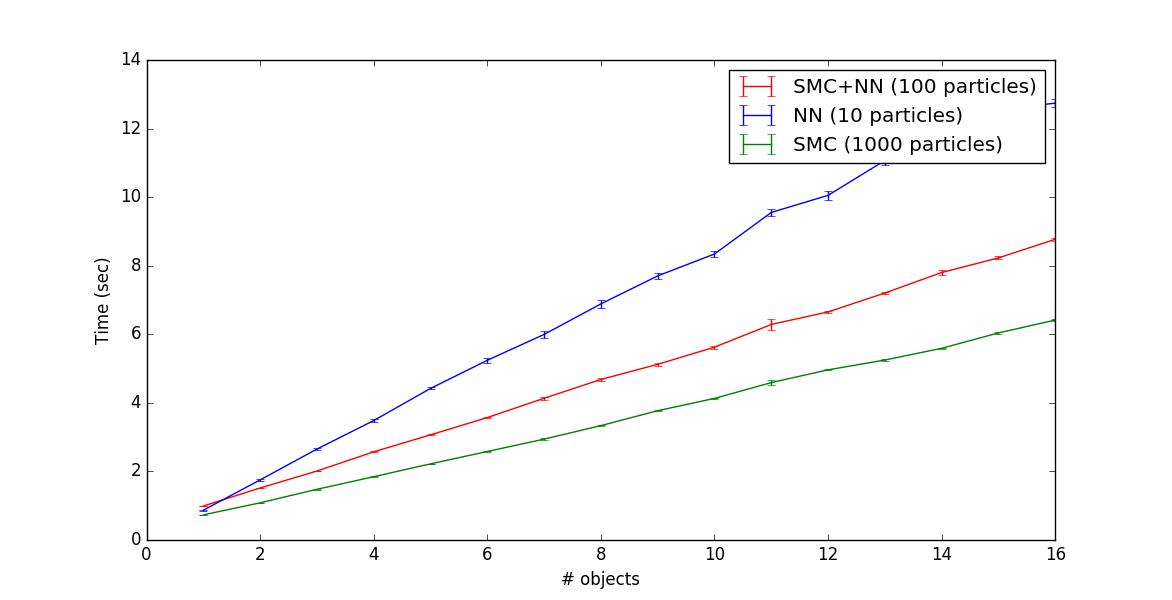
\includegraphics[width = 15cm]{figures/time.png}
  \end{minipage}
  \caption{Using the model to parse latex output. The model is trained on diagrams with up to 8 objects. As shown above it generalizes to scenes with many more objects. Neither the stochastic search nor the neural network are sufficient on their own.}\label{syntheticResults}
\end{figure}

\subsection{Generalizing to hand drawings}
We believe that converting synthetic, noiseless images into a restricted subset of
\LaTeX has limited usefulness.  A more practical
application is one that extends to hand drawings.  We train the model
to generalize to hand drawings by introducing noise into the
renderings of the training target images.
We designed this noise process to introduce the kinds of variations found in hand drawings (figure~\ref{handDrawingExamples}).
We drew 100 figures by hand; see figure~\ref{lotsOfHandDrawings}.
These were drawn reasonably carefully but not perfectly.
Because our model assumes that objects are snapped to a $16\times 16$ grid,
we made the drawings on graph paper.
\begin{figure}[H]%
  \begin{minipage}[t]{0.2\textwidth}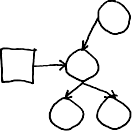
\includegraphics[width = 2cm]{figures/expert-60-reduced.png}
    \subcaption{}
  \end{minipage}%
   \begin{minipage}[t]{0.2\textwidth}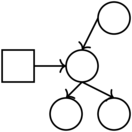
\includegraphics[width = 2cm]{figures/60-groundTruth-reduced.png}
    \subcaption{}
  \end{minipage}%
  \begin{minipage}[t]{0.2\textwidth}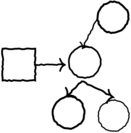
\includegraphics[width = 2cm]{figures/60-1-reduced.png}
    \subcaption{}
  \end{minipage}%
  \begin{minipage}[t]{0.2\textwidth}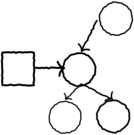
\includegraphics[width = 2cm]{figures/60-2-reduced.png} 
    \subcaption{}
  \end{minipage}
  \caption{(a): a hand drawing. (b): Rendering of the parse our model infers for (a). We can generalize to hand drawings like these because we train the model on images corrupted by a noise process designed to resemble the kind of noise introduced by hand drawings - see (c) \& (d) for noisy renderings of (b).}\ref{handDrawingExamples}
\end{figure}

\begin{figure}[H]
  \begin{minipage}[t]{2.25cm}
    
\includegraphics[width = 2cm]{figures/expert-10.png}
    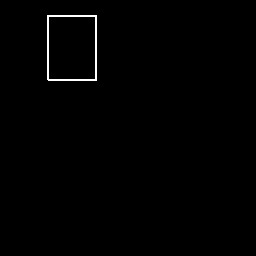
\includegraphics[width = 2cm]{figures/10-parse.png}    
    \subcaption{Noisy input}
  \end{minipage}
  \begin{minipage}[t]{2.25cm}
    \includegraphics[width = 2cm]{figures/expert-21.png}
    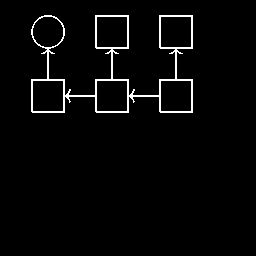
\includegraphics[width = 2cm]{figures/21-parse.png}    
    \subcaption{A graphical model}
  \end{minipage}
  \begin{minipage}[t]{2.25cm}
    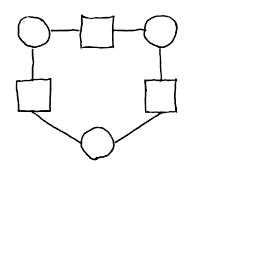
\includegraphics[width = 2cm]{figures/expert-77.png}
    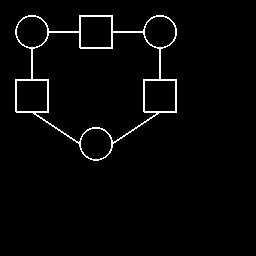
\includegraphics[width = 2cm]{figures/77-parse.png}    
    \subcaption{A figure from a deep learning textbook}
    \end{minipage}
  \begin{minipage}[t]{2.25cm}
    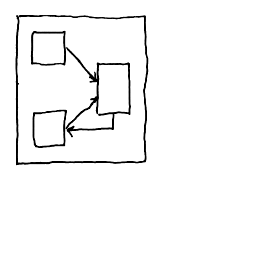
\includegraphics[width = 2cm]{figures/expert-0.png}
    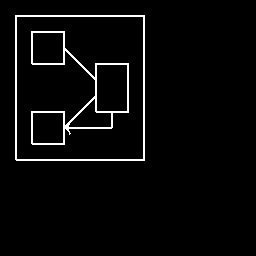
\includegraphics[width = 2cm]{figures/0-parse.png}    
    \subcaption{Near miss}
  \end{minipage}
  \begin{minipage}[t]{2.25cm}
    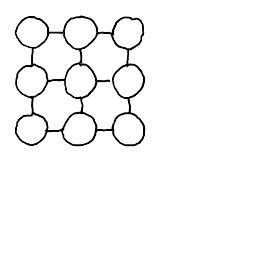
\includegraphics[width = 2cm]{figures/expert-38.png}
    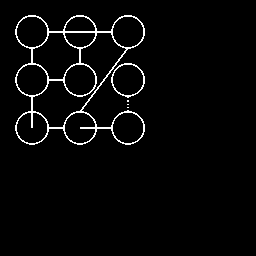
\includegraphics[width = 2cm]{figures/38-parse.png}    
    \subcaption{Failing on a Ising model}
  \end{minipage}
  \begin{minipage}[t]{2.25cm}
    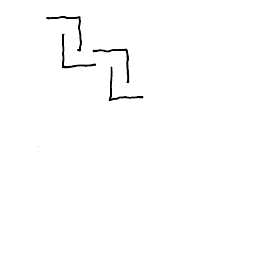
\includegraphics[width = 2cm]{figures/expert-34.png}
    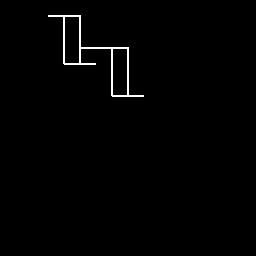
\includegraphics[width = 2cm]{figures/34-parse.png}     
    \subcaption{Illusory contours}
    \end{minipage}
  \caption{Example drawings above model outputs. See also Fig.~\ref{firstPageExamples}}\label{handDrawingExamples}
  \end{figure}

\section{Synthesizing graphics programs from execution traces}
Although the execution trace of a graphics program describes the parts
of a scene, it fails to encode higher-level features of the image,
such as repeated motifs, symmetries or reflections.  A \emph{graphics
  program} better describe structures like these,
and we now take as our goal to synthesize simple graphics programs from
their execution traces.

We constrain the space of allowed programs by writing down a context
free grammar over a space of programs. Although it might be desirable
to synthesize programs in a Turing-complete language like Lisp or
Python, a more tractable approach is to specify what in the program
languages community is called a Domain Specific Language (DSL). Our DSL (Table~\ref{DSL})
encodes prior knowledge of what graphics programs tend to look like.

\begin{table}[H]
  \begin{tabular}{rl}
  Program$\to$&Command; $\cdots$; Command\\
  Command$\to$&\texttt{circle}(Expression,Expression)\\
  Command$\to$&\texttt{rectangle}(Expression,Expression,Expression,Expression)\\
  Command$\to$&\texttt{LINE}(Expression,Expression,Expression,Expression,Boolean,Boolean)\\
  Command$\to$&\texttt{for}$(0\leq \text{Var}  < \text{Expression})$\texttt{ \{ }Program\texttt{ \}}\\
  Command$\to$&\texttt{REFLECT}$(\text{Axis})$\texttt{ \{ }Program\texttt{ \}}\\
  Expression$\to$&\mathcal{Z}\texttt{ * }Var\texttt{ + }\mathcal{Z}\\
  Var$\to$&A free (unused) variable\\
  \mathcal{Z}$\to$&an integer\\
  Axis$\to$&\texttt{X = }\mathcal{Z}\\
  Axis$\to$&\texttt{Y = }\mathcal{Z}
  \end{tabular}
  \caption{Grammar over graphics programs. We allow loops (\texttt{for}), vertical/horizontal reflections (\texttt{REFLECT}), and affine transformations (\mathcal{Z}\texttt{ * }Var\texttt{ + }\mathcal{Z}).}\label{DSL}
\end{table}

Given the DSL and a trace $T$, we want a program that evaluates to $T$
and also minimizes some measure of program cost:
\begin{equation}
  \text{program}(T) = \argmin_{\substack{p\in \text{DSL}\\p \text{ evaluates to } T}} \text{cost}(p)\label{programObjective}
\end{equation}
An intuitive measure of program cost is its length.  We define the
cost of a program to be the number of statements it contains, where a
statement is a ``Command'' in Table~\ref{DSL}.

The constrained optimization problem in
equation~\ref{programObjective} is intractable in general, but there
exist efficient-in-practice tools for finding exact solutions to
program synthesis problems like these. We use the state-of-the-art Sketch
tool~\cite{solar2008program}. Describing Sketch's program synthesis
algorithm is beyond the scope of this paper; see supplement.  At a
high level, Sketch takes as input a space of programs, along with a
specification of the program 's behavior and optionally a cost
function.  It translates the synthesis problem into a constraint
satisfaction problem, and then uses a quasiboolean solver to find a
minimum cost program satisfying the specification.  In exchange for
not having any guarantees on how long it will take to find a minimum
cost solution, it comes with the guarantee that it will always find a
globally optimal program.

Why synthesize a graphics program,
if the execution trace already suffices to recover the objects in an image?
Within our domain of hand-drawn figures, graphics program synthesis has several important uses:
\subsection{Extrapolating figures}
Given the source code of a graphics program,
we can automatically tweak the program
to make natural-feeling changes to the figure.
For example,
we can change all of the circles to squares,
were make all of the lines be dashed.
We can also \textbf{extrapolate} figures
by increasing the number of times that loops are executed.

            \begin{tabular}{ll}
    \includegraphics[width = 5cm]{../TikZ/drawings/expert-17.png}&
    \includegraphics[width = 5cm]{../TikZ/extrapolations/expert-17-extrapolation.png}
    \end{tabular}        
            \\

            \begin{tabular}{ll}
    \includegraphics[width = 5cm]{../TikZ/drawings/expert-21.png}&
    \includegraphics[width = 5cm]{../TikZ/extrapolations/expert-21-extrapolation.png}
    \end{tabular}        
            \\

            \begin{tabular}{ll}
    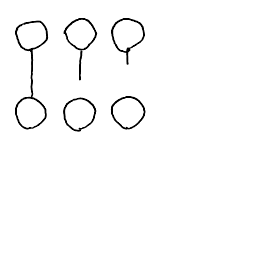
\includegraphics[width = 5cm]{../TikZ/drawings/expert-7.png}&
    \includegraphics[width = 5cm]{../TikZ/extrapolations/expert-7-extrapolation.png}
    \end{tabular}        
            \\

            \begin{tabular}{ll}
    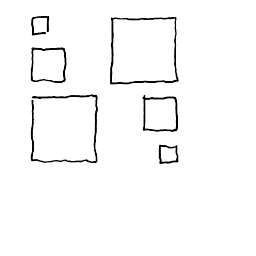
\includegraphics[width = 5cm]{../TikZ/drawings/expert-36.png}&
    \includegraphics[width = 5cm]{../TikZ/extrapolations/expert-36-extrapolation.png}
    \end{tabular}        
            \\

            \begin{tabular}{ll}
    \includegraphics[width = 5cm]{../TikZ/drawings/expert-58.png}&
    \includegraphics[width = 5cm]{../TikZ/extrapolations/expert-58-extrapolation.png}
    \end{tabular}        
            \\

            \begin{tabular}{ll}
    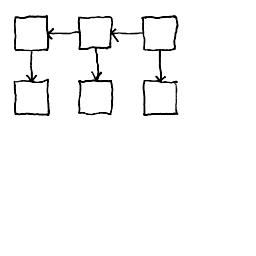
\includegraphics[width = 5cm]{../TikZ/drawings/expert-22.png}&
    \includegraphics[width = 5cm]{../TikZ/extrapolations/expert-22-extrapolation.png}
    \end{tabular}        
            \\

            \begin{tabular}{ll}
    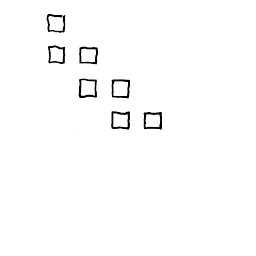
\includegraphics[width = 5cm]{../TikZ/drawings/expert-14.png}&
    \includegraphics[width = 5cm]{../TikZ/extrapolations/expert-14-extrapolation.png}
    \end{tabular}        
            \\

            \begin{tabular}{ll}
    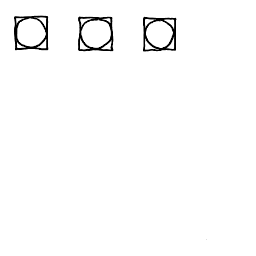
\includegraphics[width = 5cm]{../TikZ/drawings/expert-68.png}&
    \includegraphics[width = 5cm]{../TikZ/extrapolations/expert-68-extrapolation.png}
    \end{tabular}        
            \\

            \begin{tabular}{ll}
    \includegraphics[width = 5cm]{../TikZ/drawings/expert-12.png}&
    \includegraphics[width = 5cm]{../TikZ/extrapolations/expert-12-extrapolation.png}
    \end{tabular}        
            \\

            \begin{tabular}{ll}
    \includegraphics[width = 5cm]{../TikZ/drawings/expert-35.png}&
    \includegraphics[width = 5cm]{../TikZ/extrapolations/expert-35-extrapolation.png}
    \end{tabular}        
            \\

            \begin{tabular}{ll}
    \includegraphics[width = 5cm]{../TikZ/drawings/expert-31.png}&
    \includegraphics[width = 5cm]{../TikZ/extrapolations/expert-31-extrapolation.png}
    \end{tabular}        
            \\

            \begin{tabular}{ll}
    \includegraphics[width = 5cm]{../TikZ/drawings/expert-37.png}&
    \includegraphics[width = 5cm]{../TikZ/extrapolations/expert-37-extrapolation.png}
    \end{tabular}        
            \\

            \begin{tabular}{ll}
    \includegraphics[width = 5cm]{../TikZ/drawings/expert-29.png}&
    \includegraphics[width = 5cm]{../TikZ/extrapolations/expert-29-extrapolation.png}
    \end{tabular}        
            \\

            \begin{tabular}{ll}
    \includegraphics[width = 5cm]{../TikZ/drawings/expert-57.png}&
    \includegraphics[width = 5cm]{../TikZ/extrapolations/expert-57-extrapolation.png}
    \end{tabular}        
            \\

            \begin{tabular}{ll}
    \includegraphics[width = 5cm]{../TikZ/drawings/expert-23.png}&
    \includegraphics[width = 5cm]{../TikZ/extrapolations/expert-23-extrapolation.png}
    \end{tabular}        
            \\

            \begin{tabular}{ll}
    \includegraphics[width = 5cm]{../TikZ/drawings/expert-60.png}&
    \includegraphics[width = 5cm]{../TikZ/extrapolations/expert-60-extrapolation.png}
    \end{tabular}        
            \\

            \begin{tabular}{ll}
    \includegraphics[width = 5cm]{../TikZ/drawings/expert-16.png}&
    \includegraphics[width = 5cm]{../TikZ/extrapolations/expert-16-extrapolation.png}
    \end{tabular}        
            \\

            \begin{tabular}{ll}
    \includegraphics[width = 5cm]{../TikZ/drawings/expert-5.png}&
    \includegraphics[width = 5cm]{../TikZ/extrapolations/expert-5-extrapolation.png}
    \end{tabular}        
            \\

            \begin{tabular}{ll}
    \includegraphics[width = 5cm]{../TikZ/drawings/expert-50.png}&
    \includegraphics[width = 5cm]{../TikZ/extrapolations/expert-50-extrapolation.png}
    \end{tabular}        
            \\

            \begin{tabular}{ll}
    \includegraphics[width = 5cm]{../TikZ/drawings/expert-6.png}&
    \includegraphics[width = 5cm]{../TikZ/extrapolations/expert-6-extrapolation.png}
    \end{tabular}        
            

\subsection{Modeling similarity between figures}



\subsection{Correcting errors made by the neural network}

Let $L(\cdot | \cdot):\text{image}^2\to \mathcal{R}$ be our likelihood
function: it takes two images, an observed target image and a
hypothesized program output, and gives the likelihood of the observed
image conditioned on the program output.
Write $\hat{T}(I)$ for the trace the model predicts for image $I$.

We can extract a few basic features of a program, like its size or how many
loops it has,
and use these features to help predict
whether a trace is the correct explanation for an image.
\begin{equation}
\hat{T}(I) = \argmax_{T} L(I | \text{render}(T)) + \theta\cdot  \phi \left( \text{program}(T) \right)
\end{equation}
where $\phi (\cdot)$ is a feature extractor for programs.
This is equivalent to doing MAP inference in a generative model where the program
is first drawn from a log linear distribution $\propto \exp (\theta\cdot \phi (\text{program}))$,
than the program is executed deterministically,
and then we observe a noisy version of the program's output,
where $L$ is the noise model.



  \pagebreak
  \section{Preliminary extrapolation results} 



\pagebreak
  \section{Preliminary Synthesis results} 

            \begin{tabular}{lll}
    \includegraphics[width = 5cm]{../TikZ/drawings/expert-0.png}&
            \includegraphics[width = 5cm]{../TikZ/drawings/expert-0-parses/0.png}&
    
        \begin{minipage}{10cm}
        \begin{verbatim}
line(6,2,6,3,
arrow = False,solid = True);
line(6,2,3,2,
arrow = True,solid = True);
reflect(reflect(y = 9)){
line(3,2,5,4,
arrow = True,solid = True);
rectangle(0,0,8,9);
rectangle(5,3,7,6);
rectangle(1,1,3,3)
}
        \end{verbatim}
\end{minipage}

    \end{tabular}        
            \\

            \begin{tabular}{lll}
    \includegraphics[width = 5cm]{../TikZ/drawings/expert-1.png}&
            \includegraphics[width = 5cm]{../TikZ/drawings/expert-1-parses/0.png}&
    
        \begin{minipage}{10cm}
        \begin{verbatim}
Solver timeout
        \end{verbatim}
\end{minipage}

    \end{tabular}        
            \\

            \begin{tabular}{lll}
    \includegraphics[width = 5cm]{../TikZ/drawings/expert-2.png}&
            \includegraphics[width = 5cm]{../TikZ/drawings/expert-2-parses/0.png}&
    
        \begin{minipage}{10cm}
        \begin{verbatim}
rectangle(4,2,6,5);
reflect(reflect(y = 7)){
line(2,6,4,4,
arrow = True,solid = True);
rectangle(0,0,2,2)
}
        \end{verbatim}
\end{minipage}

    \end{tabular}        
            \\

            \begin{tabular}{lll}
    \includegraphics[width = 5cm]{../TikZ/drawings/expert-3.png}&
            \includegraphics[width = 5cm]{../TikZ/drawings/expert-3-parses/0.png}&
    
        \begin{minipage}{10cm}
        \begin{verbatim}
circle(10,5);
line(7,5,9,5,
arrow = True,solid = True);
rectangle(5,3,7,7);
rectangle(0,0,12,10);
reflect(reflect(y = 10)){
line(3,8,5,6,
arrow = True,solid = True);
rectangle(1,7,3,9)
}
        \end{verbatim}
\end{minipage}

    \end{tabular}        
            \\

            \begin{tabular}{lll}
    \includegraphics[width = 5cm]{../TikZ/drawings/expert-4.png}&
            \includegraphics[width = 5cm]{../TikZ/drawings/expert-4-parses/0.png}&
    
        \begin{minipage}{10cm}
        \begin{verbatim}
circle(10,4);
line(10,1,2,1,
arrow = True,solid = False);
line(10,1,10,3,
arrow = False,solid = False);
line(7,4,9,4,
arrow = True,solid = True);
reflect(reflect(y = 8)){
line(2,7,4,5,
arrow = True,solid = True);
rectangle(4,2,7,6);
rectangle(0,6,2,8)
}
        \end{verbatim}
\end{minipage}

    \end{tabular}        
            \\

            \begin{tabular}{lll}
    \includegraphics[width = 5cm]{../TikZ/drawings/expert-5.png}&
            \includegraphics[width = 5cm]{../TikZ/drawings/expert-5-parses/0.png}&
    
        \begin{minipage}{10cm}
        \begin{verbatim}
Solver timeout
        \end{verbatim}
\end{minipage}

    \end{tabular}        
            \\

            \begin{tabular}{lll}
    \includegraphics[width = 5cm]{../TikZ/drawings/expert-6.png}&
            \includegraphics[width = 5cm]{../TikZ/drawings/expert-6-parses/0.png}&
    
        \begin{minipage}{10cm}
        \begin{verbatim}
line(0,1,2,0,
arrow = False,solid = True);
for (i < 3){
if (i > 0){
line(3*i + -3,4,3*i + -1,3,
arrow = False,solid = True);
line(0,3*i + -2,3*i + -3,4,
arrow = False,solid = True)
}
rectangle(2,0,5,3)
}
        \end{verbatim}
\end{minipage}

    \end{tabular}        
            \\

            \begin{tabular}{lll}
    \includegraphics[width = 5cm]{../TikZ/drawings/expert-7.png}&
            \includegraphics[width = 5cm]{../TikZ/drawings/expert-7-parses/0.png}&
    
        \begin{minipage}{10cm}
        \begin{verbatim}
for (i < 3){
circle(-3*i + 7,1);
circle(-3*i + 7,6);
line(-3*i + 7,-1*i + 4,-3*i + 7,5,
arrow = False,solid = True)
}
        \end{verbatim}
\end{minipage}

    \end{tabular}        
            \\

            \begin{tabular}{lll}
    \includegraphics[width = 5cm]{../TikZ/drawings/expert-8.png}&
            \includegraphics[width = 5cm]{../TikZ/drawings/expert-8-parses/0.png}&
    
        \begin{minipage}{10cm}
        \begin{verbatim}
line(0,0,0,4,
arrow = False,solid = True)
        \end{verbatim}
\end{minipage}

    \end{tabular}        
            \\

            \begin{tabular}{lll}
    \includegraphics[width = 5cm]{../TikZ/drawings/expert-9.png}&
            \includegraphics[width = 5cm]{../TikZ/drawings/expert-9-parses/0.png}&
    
        \begin{minipage}{10cm}
        \begin{verbatim}
line(6,0,0,0,
arrow = True,solid = True)
        \end{verbatim}
\end{minipage}

    \end{tabular}        
            \\

            \begin{tabular}{lll}
    \includegraphics[width = 5cm]{../TikZ/drawings/expert-10.png}&
            \includegraphics[width = 5cm]{../TikZ/drawings/expert-10-parses/0.png}&
    
        \begin{minipage}{10cm}
        \begin{verbatim}
rectangle(0,0,3,4)
        \end{verbatim}
\end{minipage}

    \end{tabular}        
            \\

            \begin{tabular}{lll}
    \includegraphics[width = 5cm]{../TikZ/drawings/expert-11.png}&
            \includegraphics[width = 5cm]{../TikZ/drawings/expert-11-parses/0.png}&
    
        \begin{minipage}{10cm}
        \begin{verbatim}
circle(1,1)
        \end{verbatim}
\end{minipage}

    \end{tabular}        
            \\

            \begin{tabular}{lll}
    \includegraphics[width = 5cm]{../TikZ/drawings/expert-12.png}&
            \includegraphics[width = 5cm]{../TikZ/drawings/expert-12-parses/0.png}&
    
        \begin{minipage}{10cm}
        \begin{verbatim}
line(2,6,5,6,
arrow = False,solid = True);
reflect(reflect(x = 7)){
circle(6,1);
line(2,1,5,1,
arrow = False,solid = True);
line(1,2,1,5,
arrow = False,solid = True);
rectangle(5,5,7,7)
}
        \end{verbatim}
\end{minipage}

    \end{tabular}        
            \\

            \begin{tabular}{lll}
    \includegraphics[width = 5cm]{../TikZ/drawings/expert-13.png}&
            \includegraphics[width = 5cm]{../TikZ/drawings/expert-13-parses/0.png}&
    
        \begin{minipage}{10cm}
        \begin{verbatim}
line(2,1,4,1,
arrow = True,solid = True);
line(3,2,1,2,
arrow = True,solid = True);
line(5,0,3,0,
arrow = True,solid = True);
line(0,3,2,3,
arrow = True,solid = True)
        \end{verbatim}
\end{minipage}

    \end{tabular}        
            \\

            \begin{tabular}{lll}
    \includegraphics[width = 5cm]{../TikZ/drawings/expert-14.png}&
            \includegraphics[width = 5cm]{../TikZ/drawings/expert-14-parses/0.png}&
    
        \begin{minipage}{10cm}
        \begin{verbatim}
for (i < 4){
if (i > 0){
rectangle(-2*i + 6,2*i + -2,-2*i + 7,2*i + -1)
}
rectangle(-2*i + 6,2*i,-2*i + 7,2*i + 1)
}
        \end{verbatim}
\end{minipage}

    \end{tabular}        
            \\

            \begin{tabular}{lll}
    \includegraphics[width = 5cm]{../TikZ/drawings/expert-15.png}&
            \includegraphics[width = 5cm]{../TikZ/drawings/expert-15-parses/0.png}&
    
        \begin{minipage}{10cm}
        \begin{verbatim}
line(0,3,2,3,
arrow = False,solid = False);
line(2,1,4,1,
arrow = False,solid = False);
line(1,2,3,2,
arrow = False,solid = True);
line(3,0,5,0,
arrow = False,solid = True)
        \end{verbatim}
\end{minipage}

    \end{tabular}        
            \\

            \begin{tabular}{lll}
    \includegraphics[width = 5cm]{../TikZ/drawings/expert-16.png}&
            \includegraphics[width = 5cm]{../TikZ/drawings/expert-16-parses/0.png}&
    
        \begin{minipage}{10cm}
        \begin{verbatim}
for (i < 4){
if (i > 0){
circle(-2*i + 7,3*i + -2);
line(-2*i + 9,3*i,-2*i + 10,3*i + -2,
arrow = False,solid = True);
line(-2*i + 8,3*i + -2,-2*i + 9,3*i,
arrow = False,solid = True)
}
circle(-2*i + 9,3*i + 1)
}
        \end{verbatim}
\end{minipage}

    \end{tabular}        
            \\

            \begin{tabular}{lll}
    \includegraphics[width = 5cm]{../TikZ/drawings/expert-17.png}&
            \includegraphics[width = 5cm]{../TikZ/drawings/expert-17-parses/0.png}&
    
        \begin{minipage}{10cm}
        \begin{verbatim}
for (i < 4){
if (i > 0){
line(2*i + 1,-3*i + 12,2*i,-3*i + 10,
arrow = True,solid = True);
line(2*i + 1,-3*i + 12,2*i + 2,-3*i + 10,
arrow = True,solid = True);
rectangle(2*i + -2,-3*i + 9,2*i,-3*i + 11)
}
rectangle(2*i + 2,-3*i + 9,2*i + 4,-3*i + 11)
}
        \end{verbatim}
\end{minipage}

    \end{tabular}        
            \\

            \begin{tabular}{lll}
    \includegraphics[width = 5cm]{../TikZ/drawings/expert-18.png}&
            \includegraphics[width = 5cm]{../TikZ/drawings/expert-18-parses/0.png}&
    
        \begin{minipage}{10cm}
        \begin{verbatim}
circle(5,1);
for (i < 3){
if (i > 0){
circle(7,2*i + -1);
circle(i + 2,2*i + 1)
}
circle(1,6)
}
        \end{verbatim}
\end{minipage}

    \end{tabular}        
            \\

            \begin{tabular}{lll}
    \includegraphics[width = 5cm]{../TikZ/drawings/expert-19.png}&
            \includegraphics[width = 5cm]{../TikZ/drawings/expert-19-parses/0.png}&
    
        \begin{minipage}{10cm}
        \begin{verbatim}
line(4,4,2,2,
arrow = True,solid = True);
rectangle(3,4,5,6);
rectangle(0,0,2,2)
        \end{verbatim}
\end{minipage}

    \end{tabular}        
            \\

            \begin{tabular}{lll}
    \includegraphics[width = 5cm]{../TikZ/drawings/expert-20.png}&
            \includegraphics[width = 5cm]{../TikZ/drawings/expert-20-parses/0.png}&
    
        \begin{minipage}{10cm}
        \begin{verbatim}
rectangle(0,4,2,6);
for (i < 3){
if (i > 0){
line(-4*i + 12,5,-4*i + 10,5,
arrow = True,solid = True);
for (j < i + 1){
circle(-4*j + 9,-4*i + 9)
}
}
line(-4*i + 9,4,-4*i + 9,2,
arrow = True,solid = True)
}
        \end{verbatim}
\end{minipage}

    \end{tabular}        
            \\

            \begin{tabular}{lll}
    \includegraphics[width = 5cm]{../TikZ/drawings/expert-21.png}&
            \includegraphics[width = 5cm]{../TikZ/drawings/expert-21-parses/0.png}&
    
        \begin{minipage}{10cm}
        \begin{verbatim}
Solver timeout
        \end{verbatim}
\end{minipage}

    \end{tabular}        
            \\

            \begin{tabular}{lll}
    \includegraphics[width = 5cm]{../TikZ/drawings/expert-22.png}&
            \includegraphics[width = 5cm]{../TikZ/drawings/expert-22-parses/0.png}&
    
        \begin{minipage}{10cm}
        \begin{verbatim}
for (i < 3){
line(-4*i + 9,4,-4*i + 9,2,
arrow = True,solid = True);
for (j < 2){
line(-4*j + 8,5,-4*j + 6,5,
arrow = True,solid = True);
rectangle(-4*i + 8,4*j,-4*i + 10,4*j + 2)
}
}
        \end{verbatim}
\end{minipage}

    \end{tabular}        
            \\

            \begin{tabular}{lll}
    \includegraphics[width = 5cm]{../TikZ/drawings/expert-23.png}&
            \includegraphics[width = 5cm]{../TikZ/drawings/expert-23-parses/0.png}&
    
        \begin{minipage}{10cm}
        \begin{verbatim}
for (i < 3){
if (i > 0){
line(-4*i + 12,1,-4*i + 10,1,
arrow = True,solid = True)
}
circle(-4*i + 9,1);
circle(-4*i + 9,5);
line(-4*i + 9,2,-4*i + 9,4,
arrow = True,solid = True)
}
        \end{verbatim}
\end{minipage}

    \end{tabular}        
            \\

            \begin{tabular}{lll}
    \includegraphics[width = 5cm]{../TikZ/drawings/expert-24.png}&
            \includegraphics[width = 5cm]{../TikZ/drawings/expert-24-parses/0.png}&
    
        \begin{minipage}{10cm}
        \begin{verbatim}
reflect(reflect(x = 6)){
for (i < 3){
if (i > 0){
line(-2*i + 7,-4*i + 11,-2*i + 7,-4*i + 10,
arrow = True,solid = True);
rectangle(0,-4*i + 11,6,-3*i + 12)
}
rectangle(2,0,4,2)
}
}
        \end{verbatim}
\end{minipage}

    \end{tabular}        
            \\

            \begin{tabular}{lll}
    \includegraphics[width = 5cm]{../TikZ/drawings/expert-25.png}&
            \includegraphics[width = 5cm]{../TikZ/drawings/expert-25-parses/0.png}&
    
        \begin{minipage}{10cm}
        \begin{verbatim}
for (i < 3){
if (i > 0){
line(3*i,1,3*i + -1,1,
arrow = True,solid = True)
}
rectangle(3*i,0,3*i + 2,2)
}
        \end{verbatim}
\end{minipage}

    \end{tabular}        
            \\

            \begin{tabular}{lll}
    \includegraphics[width = 5cm]{../TikZ/drawings/expert-26.png}&
            \includegraphics[width = 5cm]{../TikZ/drawings/expert-26-parses/0.png}&
    
        \begin{minipage}{10cm}
        \begin{verbatim}
line(1,3,1,4,
arrow = False,solid = True);
for (i < 3){
if (i > 0){
line(1,-5*i + 13,1,-4*i + 10,
arrow = True,solid = True)
}
circle(1,-4*i + 9)
}
        \end{verbatim}
\end{minipage}

    \end{tabular}        
            \\

            \begin{tabular}{lll}
    \includegraphics[width = 5cm]{../TikZ/drawings/expert-27.png}&
            \includegraphics[width = 5cm]{../TikZ/drawings/expert-27-parses/0.png}&
    
        \begin{minipage}{10cm}
        \begin{verbatim}
reflect(reflect(x = 2)){
line(0,1,1,2,
arrow = False,solid = True);
line(1,0,2,1,
arrow = False,solid = True)
}
        \end{verbatim}
\end{minipage}

    \end{tabular}        
            \\

            \begin{tabular}{lll}
    \includegraphics[width = 5cm]{../TikZ/drawings/expert-28.png}&
            \includegraphics[width = 5cm]{../TikZ/drawings/expert-28-parses/0.png}&
    
        \begin{minipage}{10cm}
        \begin{verbatim}
line(0,0,0,2,
arrow = False,solid = True);
line(0,2,2,2,
arrow = False,solid = True)
        \end{verbatim}
\end{minipage}

    \end{tabular}        
            \\

            \begin{tabular}{lll}
    \includegraphics[width = 5cm]{../TikZ/drawings/expert-29.png}&
            \includegraphics[width = 5cm]{../TikZ/drawings/expert-29-parses/0.png}&
    
        \begin{minipage}{10cm}
        \begin{verbatim}
for (i < 3){
line(i,-1*i + 6,2*i + 2,-1*i + 6,
arrow = False,solid = True);
line(i,-2*i + 4,i,-1*i + 6,
arrow = False,solid = True)
}
        \end{verbatim}
\end{minipage}

    \end{tabular}        
            \\

            \begin{tabular}{lll}
    \includegraphics[width = 5cm]{../TikZ/drawings/expert-30.png}&
            \includegraphics[width = 5cm]{../TikZ/drawings/expert-30-parses/0.png}&
    
        \begin{minipage}{10cm}
        \begin{verbatim}
for (i < 3){
if (i > 0){
circle(1,-3*i + 7);
circle(5,-2*i + 6);
rectangle(0,-3*i + 6,2,-3*i + 8)
}
rectangle(4,1,6,5)
}
        \end{verbatim}
\end{minipage}

    \end{tabular}        
            \\

            \begin{tabular}{lll}
    \includegraphics[width = 5cm]{../TikZ/drawings/expert-31.png}&
            \includegraphics[width = 5cm]{../TikZ/drawings/expert-31-parses/0.png}&
    
        \begin{minipage}{10cm}
        \begin{verbatim}
for (i < 3){
rectangle(3*i,-2*i + 4,3*i + 2,6);
for (j < i + 1){
circle(3*i + 1,-2*j + 5)
}
}
        \end{verbatim}
\end{minipage}

    \end{tabular}        
            \\

            \begin{tabular}{lll}
    \includegraphics[width = 5cm]{../TikZ/drawings/expert-32.png}&
            \includegraphics[width = 5cm]{../TikZ/drawings/expert-32-parses/0.png}&
    
        \begin{minipage}{10cm}
        \begin{verbatim}
circle(5,5);
line(2,5,4,5,
arrow = False,solid = True);
rectangle(0,0,5,3);
rectangle(0,4,2,6)
        \end{verbatim}
\end{minipage}

    \end{tabular}        
            \\

            \begin{tabular}{lll}
    \includegraphics[width = 5cm]{../TikZ/drawings/expert-33.png}&
            \includegraphics[width = 5cm]{../TikZ/drawings/expert-33-parses/0.png}&
    
        \begin{minipage}{10cm}
        \begin{verbatim}
line(0,0,6,0,
arrow = False,solid = False);
reflect(reflect(x = 6)){
line(6,0,6,3,
arrow = False,solid = True);
line(0,3,6,3,
arrow = False,solid = False)
}
        \end{verbatim}
\end{minipage}

    \end{tabular}        
            \\

            \begin{tabular}{lll}
    \includegraphics[width = 5cm]{../TikZ/drawings/expert-34.png}&
            \includegraphics[width = 5cm]{../TikZ/drawings/expert-34-parses/0.png}&
    
        \begin{minipage}{10cm}
        \begin{verbatim}
Solver timeout
        \end{verbatim}
\end{minipage}

    \end{tabular}        
            \\

            \begin{tabular}{lll}
    \includegraphics[width = 5cm]{../TikZ/drawings/expert-35.png}&
            \includegraphics[width = 5cm]{../TikZ/drawings/expert-35-parses/0.png}&
    
        \begin{minipage}{10cm}
        \begin{verbatim}
for (i < 3){
if (i > 0){
circle(-5*i + 11,1);
line(-1*i + 3,-1*i + 7,-5*i + 11,2,
arrow = True,solid = True)
}
circle(1,6)
}
        \end{verbatim}
\end{minipage}

    \end{tabular}        
            \\

            \begin{tabular}{lll}
    \includegraphics[width = 5cm]{../TikZ/drawings/expert-36.png}&
            \includegraphics[width = 5cm]{../TikZ/drawings/expert-36-parses/0.png}&
    
        \begin{minipage}{10cm}
        \begin{verbatim}
Solver timeout
        \end{verbatim}
\end{minipage}

    \end{tabular}        
            \\

            \begin{tabular}{lll}
    \includegraphics[width = 5cm]{../TikZ/drawings/expert-37.png}&
            \includegraphics[width = 5cm]{../TikZ/drawings/expert-37-parses/0.png}&
    
        \begin{minipage}{10cm}
        \begin{verbatim}
for (i < 3){
if (i > 0){
line(4*i + -3,-5*i + 12,2*i + 1,5,
arrow = False,solid = True);
rectangle(4*i + -4,-5*i + 10,6,-7*i + 16)
}
circle(1,8)
}
        \end{verbatim}
\end{minipage}

    \end{tabular}        
            \\

            \begin{tabular}{lll}
    \includegraphics[width = 5cm]{../TikZ/drawings/expert-38.png}&
            \includegraphics[width = 5cm]{../TikZ/drawings/expert-38-parses/0.png}&
    
        \begin{minipage}{10cm}
        \begin{verbatim}
Solver timeout
        \end{verbatim}
\end{minipage}

    \end{tabular}        
            \\

            \begin{tabular}{lll}
    \includegraphics[width = 5cm]{../TikZ/drawings/expert-39.png}&
            \includegraphics[width = 5cm]{../TikZ/drawings/expert-39-parses/0.png}&
    
        \begin{minipage}{10cm}
        \begin{verbatim}
Solver timeout
        \end{verbatim}
\end{minipage}

    \end{tabular}        
            \\

            \begin{tabular}{lll}
    \includegraphics[width = 5cm]{../TikZ/drawings/expert-40.png}&
            \includegraphics[width = 5cm]{../TikZ/drawings/expert-40-parses/0.png}&
    
        \begin{minipage}{10cm}
        \begin{verbatim}
for (i < 3){
circle(-3*i + 7,1)
}
        \end{verbatim}
\end{minipage}

    \end{tabular}        
            \\

            \begin{tabular}{lll}
    \includegraphics[width = 5cm]{../TikZ/drawings/expert-41.png}&
            \includegraphics[width = 5cm]{../TikZ/drawings/expert-41-parses/0.png}&
    
        \begin{minipage}{10cm}
        \begin{verbatim}
for (i < 3){
rectangle(-2*i + 4,0,-2*i + 5,6)
}
        \end{verbatim}
\end{minipage}

    \end{tabular}        
            \\

            \begin{tabular}{lll}
    \includegraphics[width = 5cm]{../TikZ/drawings/expert-42.png}&
            \includegraphics[width = 5cm]{../TikZ/drawings/expert-42-parses/0.png}&
    
        \begin{minipage}{10cm}
        \begin{verbatim}
line(4,0,4,1,
arrow = False,solid = False);
line(0,0,0,5,
arrow = False,solid = False);
line(4,1,4,5,
arrow = False,solid = False)
        \end{verbatim}
\end{minipage}

    \end{tabular}        
            \\

            \begin{tabular}{lll}
    \includegraphics[width = 5cm]{../TikZ/drawings/expert-43.png}&
            \includegraphics[width = 5cm]{../TikZ/drawings/expert-43-parses/0.png}&
    
        \begin{minipage}{10cm}
        \begin{verbatim}
line(4,0,4,5,
arrow = False,solid = True);
line(0,0,0,5,
arrow = False,solid = True)
        \end{verbatim}
\end{minipage}

    \end{tabular}        
            \\

            \begin{tabular}{lll}
    \includegraphics[width = 5cm]{../TikZ/drawings/expert-44.png}&
            \includegraphics[width = 5cm]{../TikZ/drawings/expert-44-parses/0.png}&
    
        \begin{minipage}{10cm}
        \begin{verbatim}
reflect(reflect(x = 12)){
circle(4,1);
line(9,1,10,1,
arrow = False,solid = True);
rectangle(0,0,2,2)
}
        \end{verbatim}
\end{minipage}

    \end{tabular}        
            \\

            \begin{tabular}{lll}
    \includegraphics[width = 5cm]{../TikZ/drawings/expert-45.png}&
            \includegraphics[width = 5cm]{../TikZ/drawings/expert-45-parses/0.png}&
    
        \begin{minipage}{10cm}
        \begin{verbatim}
rectangle(0,4,4,8);
reflect(reflect(y = 12)){
circle(7,6);
line(2,2,2,4,
arrow = True,solid = True);
line(4,6,6,6,
arrow = True,solid = True);
rectangle(1,10,3,12)
}
        \end{verbatim}
\end{minipage}

    \end{tabular}        
            \\

            \begin{tabular}{lll}
    \includegraphics[width = 5cm]{../TikZ/drawings/expert-46.png}&
            \includegraphics[width = 5cm]{../TikZ/drawings/expert-46-parses/0.png}&
    
        \begin{minipage}{10cm}
        \begin{verbatim}
reflect(reflect(y = 9)){
line(3,8,6,8,
arrow = False,solid = True);
reflect(reflect(x = 9)){
circle(1,8);
line(1,3,1,6,
arrow = False,solid = True)
}
}
        \end{verbatim}
\end{minipage}

    \end{tabular}        
            \\

            \begin{tabular}{lll}
    \includegraphics[width = 5cm]{../TikZ/drawings/expert-47.png}&
            \includegraphics[width = 5cm]{../TikZ/drawings/expert-47-parses/0.png}&
    
        \begin{minipage}{10cm}
        \begin{verbatim}
reflect(reflect(y = 11)){
rectangle(4,9,7,10);
reflect(reflect(x = 11)){
rectangle(1,4,2,7);
rectangle(8,8,11,11)
}
}
        \end{verbatim}
\end{minipage}

    \end{tabular}        
            \\

            \begin{tabular}{lll}
    \includegraphics[width = 5cm]{../TikZ/drawings/expert-48.png}&
            \includegraphics[width = 5cm]{../TikZ/drawings/expert-48-parses/0.png}&
    
        \begin{minipage}{10cm}
        \begin{verbatim}
for (i < 4){
line(i,-1*i + 5,i + 2,-1*i + 5,
arrow = False,solid = True);
line(i + 2,-1*i + 3,i + 4,-1*i + 3,
arrow = False,solid = True)
}
        \end{verbatim}
\end{minipage}

    \end{tabular}        
            \\

            \begin{tabular}{lll}
    \includegraphics[width = 5cm]{../TikZ/drawings/expert-49.png}&
            \includegraphics[width = 5cm]{../TikZ/drawings/expert-49-parses/0.png}&
    
        \begin{minipage}{10cm}
        \begin{verbatim}
for (i < 3){
if (i > 0){
rectangle(3*i + 1,-1*i + 2,3*i + 3,2);
rectangle(0,7*i + -7,3,7*i + -4)
}
rectangle(1,4,2,6)
}
        \end{verbatim}
\end{minipage}

    \end{tabular}        
            \\

            \begin{tabular}{lll}
    \includegraphics[width = 5cm]{../TikZ/drawings/expert-50.png}&
            \includegraphics[width = 5cm]{../TikZ/drawings/expert-50-parses/0.png}&
    
        \begin{minipage}{10cm}
        \begin{verbatim}
Solver timeout
        \end{verbatim}
\end{minipage}

    \end{tabular}        
            \\

            \begin{tabular}{lll}
    \includegraphics[width = 5cm]{../TikZ/drawings/expert-51.png}&
            \includegraphics[width = 5cm]{../TikZ/drawings/expert-51-parses/0.png}&
    
        \begin{minipage}{10cm}
        \begin{verbatim}
for (i < 3){
rectangle(-2*i + 4,-2*i + 4,-2*i + 7,-2*i + 5)
}
        \end{verbatim}
\end{minipage}

    \end{tabular}        
            \\

            \begin{tabular}{lll}
    \includegraphics[width = 5cm]{../TikZ/drawings/expert-52.png}&
            \includegraphics[width = 5cm]{../TikZ/drawings/expert-52-parses/0.png}&
    
        \begin{minipage}{10cm}
        \begin{verbatim}
circle(4,10);
for (i < 3){
circle(-3*i + 7,5);
circle(-3*i + 7,1);
line(-3*i + 7,4,-3*i + 7,2,
arrow = True,solid = True);
line(4,9,-3*i + 7,6,
arrow = True,solid = True)
}
        \end{verbatim}
\end{minipage}

    \end{tabular}        
            \\

            \begin{tabular}{lll}
    \includegraphics[width = 5cm]{../TikZ/drawings/expert-53.png}&
            \includegraphics[width = 5cm]{../TikZ/drawings/expert-53-parses/0.png}&
    
        \begin{minipage}{10cm}
        \begin{verbatim}
line(2,8,2,6,
arrow = True,solid = True);
line(6,8,6,4,
arrow = True,solid = True);
line(4,8,4,0,
arrow = True,solid = True);
line(0,8,8,8,
arrow = False,solid = True)
        \end{verbatim}
\end{minipage}

    \end{tabular}        
            \\

            \begin{tabular}{lll}
    \includegraphics[width = 5cm]{../TikZ/drawings/expert-54.png}&
            \includegraphics[width = 5cm]{../TikZ/drawings/expert-54-parses/0.png}&
    
        \begin{minipage}{10cm}
        \begin{verbatim}
line(2,3,2,5,
arrow = False,solid = True);
rectangle(1,1,3,3);
rectangle(1,5,3,7);
rectangle(0,0,4,8)
        \end{verbatim}
\end{minipage}

    \end{tabular}        
            \\

            \begin{tabular}{lll}
    \includegraphics[width = 5cm]{../TikZ/drawings/expert-55.png}&
            \includegraphics[width = 5cm]{../TikZ/drawings/expert-55-parses/0.png}&
    
        \begin{minipage}{10cm}
        \begin{verbatim}
circle(1,5);
line(1,4,1,2,
arrow = True,solid = True);
rectangle(0,0,2,2)
        \end{verbatim}
\end{minipage}

    \end{tabular}        
            \\

            \begin{tabular}{lll}
    \includegraphics[width = 5cm]{../TikZ/drawings/expert-56.png}&
            \includegraphics[width = 5cm]{../TikZ/drawings/expert-56-parses/0.png}&
    
        \begin{minipage}{10cm}
        \begin{verbatim}
Solver timeout
        \end{verbatim}
\end{minipage}

    \end{tabular}        
            \\

            \begin{tabular}{lll}
    \includegraphics[width = 5cm]{../TikZ/drawings/expert-57.png}&
            \includegraphics[width = 5cm]{../TikZ/drawings/expert-57-parses/0.png}&
    
        \begin{minipage}{10cm}
        \begin{verbatim}
for (i < 3){
for (j < 3){
circle(-4*j + 9,-3*i + 7)
}
}
        \end{verbatim}
\end{minipage}

    \end{tabular}        
            \\

            \begin{tabular}{lll}
    \includegraphics[width = 5cm]{../TikZ/drawings/expert-58.png}&
            \includegraphics[width = 5cm]{../TikZ/drawings/expert-58-parses/0.png}&
    
        \begin{minipage}{10cm}
        \begin{verbatim}
for (i < 3){
if (i > 0){
line(8,0,8*i + -8,7*i + -7,
arrow = True,solid = True)
}
rectangle(2*i + 2,0,2*i + 3,i + 3)
}
        \end{verbatim}
\end{minipage}

    \end{tabular}        
            \\

            \begin{tabular}{lll}
    \includegraphics[width = 5cm]{../TikZ/drawings/expert-59.png}&
            \includegraphics[width = 5cm]{../TikZ/drawings/expert-59-parses/0.png}&
    
        \begin{minipage}{10cm}
        \begin{verbatim}
line(4,0,0,0,
arrow = False,solid = False)
        \end{verbatim}
\end{minipage}

    \end{tabular}        
            \\

            \begin{tabular}{lll}
    \includegraphics[width = 5cm]{../TikZ/drawings/expert-60.png}&
            \includegraphics[width = 5cm]{../TikZ/drawings/expert-60-parses/0.png}&
    
        \begin{minipage}{10cm}
        \begin{verbatim}
Solver timeout
        \end{verbatim}
\end{minipage}

    \end{tabular}        
            \\

            \begin{tabular}{lll}
    \includegraphics[width = 5cm]{../TikZ/drawings/expert-61.png}&
            \includegraphics[width = 5cm]{../TikZ/drawings/expert-61-parses/0.png}&
    
        \begin{minipage}{10cm}
        \begin{verbatim}
circle(2,1);
circle(6,1);
line(5,1,3,1,
arrow = True,solid = True);
rectangle(0,0,7,2)
        \end{verbatim}
\end{minipage}

    \end{tabular}        
            \\

            \begin{tabular}{lll}
    \includegraphics[width = 5cm]{../TikZ/drawings/expert-62.png}&
            \includegraphics[width = 5cm]{../TikZ/drawings/expert-62-parses/0.png}&
    
        \begin{minipage}{10cm}
        \begin{verbatim}
rectangle(5,0,8,3);
rectangle(2,1,4,3);
rectangle(0,2,1,3)
        \end{verbatim}
\end{minipage}

    \end{tabular}        
            \\

            \begin{tabular}{lll}
    \includegraphics[width = 5cm]{../TikZ/drawings/expert-63.png}&
            \includegraphics[width = 5cm]{../TikZ/drawings/expert-63-parses/0.png}&
    
        \begin{minipage}{10cm}
        \begin{verbatim}
for (i < 3){
rectangle(-1*i + 2,-1*i + 2,i + 3,i + 3)
}
        \end{verbatim}
\end{minipage}

    \end{tabular}        
            \\

            \begin{tabular}{lll}
    \includegraphics[width = 5cm]{../TikZ/drawings/expert-64.png}&
            \includegraphics[width = 5cm]{../TikZ/drawings/expert-64-parses/0.png}&
    
        \begin{minipage}{10cm}
        \begin{verbatim}
reflect(reflect(x = 6)){
line(5,2,5,4,
arrow = False,solid = True);
reflect(reflect(y = 6)){
line(2,1,4,1,
arrow = False,solid = True);
rectangle(4,4,6,6)
}
}
        \end{verbatim}
\end{minipage}

    \end{tabular}        
            \\

            \begin{tabular}{lll}
    \includegraphics[width = 5cm]{../TikZ/drawings/expert-65.png}&
            \includegraphics[width = 5cm]{../TikZ/drawings/expert-65-parses/0.png}&
    
        \begin{minipage}{10cm}
        \begin{verbatim}
reflect(reflect(y = 6)){
line(2,5,4,5,
arrow = False,solid = True);
reflect(reflect(x = 6)){
circle(5,5);
line(1,2,1,4,
arrow = False,solid = True)
}
}
        \end{verbatim}
\end{minipage}

    \end{tabular}        
            \\

            \begin{tabular}{lll}
    \includegraphics[width = 5cm]{../TikZ/drawings/expert-66.png}&
            \includegraphics[width = 5cm]{../TikZ/drawings/expert-66-parses/0.png}&
    
        \begin{minipage}{10cm}
        \begin{verbatim}
for (i < 3){
line(i,-1*i + 2,-1*i + 7,-1*i + 2,
arrow = False,solid = True)
}
        \end{verbatim}
\end{minipage}

    \end{tabular}        
            \\

            \begin{tabular}{lll}
    \includegraphics[width = 5cm]{../TikZ/drawings/expert-67.png}&
            \includegraphics[width = 5cm]{../TikZ/drawings/expert-67-parses/0.png}&
    
        \begin{minipage}{10cm}
        \begin{verbatim}
line(1,4,5,0,
arrow = False,solid = True);
line(1,5,5,1,
arrow = False,solid = True);
rectangle(5,0,6,1);
rectangle(0,4,1,5)
        \end{verbatim}
\end{minipage}

    \end{tabular}        
            \\

            \begin{tabular}{lll}
    \includegraphics[width = 5cm]{../TikZ/drawings/expert-68.png}&
            \includegraphics[width = 5cm]{../TikZ/drawings/expert-68-parses/0.png}&
    
        \begin{minipage}{10cm}
        \begin{verbatim}
for (i < 3){
circle(4*i + 1,1);
rectangle(4*i,0,4*i + 2,2)
}
        \end{verbatim}
\end{minipage}

    \end{tabular}        
            \\

            \begin{tabular}{lll}
    \includegraphics[width = 5cm]{../TikZ/drawings/expert-69.png}&
            \includegraphics[width = 5cm]{../TikZ/drawings/expert-69-parses/0.png}&
    
        \begin{minipage}{10cm}
        \begin{verbatim}
reflect(reflect(x = 5)){
circle(1,1);
line(4,4,4,2,
arrow = True,solid = True);
rectangle(0,4,5,6)
}
        \end{verbatim}
\end{minipage}

    \end{tabular}        
            \\

            \begin{tabular}{lll}
    \includegraphics[width = 5cm]{../TikZ/drawings/expert-70.png}&
            \includegraphics[width = 5cm]{../TikZ/drawings/expert-70-parses/0.png}&
    
        \begin{minipage}{10cm}
        \begin{verbatim}
Solver timeout
        \end{verbatim}
\end{minipage}

    \end{tabular}        
            \\

            \begin{tabular}{lll}
    \includegraphics[width = 5cm]{../TikZ/drawings/expert-71.png}&
            Sampled no finished traces.&
    
        \begin{minipage}{10cm}
        \begin{verbatim}
Solver timeout
        \end{verbatim}
\end{minipage}

    \end{tabular}        
            \\

            \begin{tabular}{lll}
    \includegraphics[width = 5cm]{../TikZ/drawings/expert-72.png}&
            \includegraphics[width = 5cm]{../TikZ/drawings/expert-72-parses/0.png}&
    
        \begin{minipage}{10cm}
        \begin{verbatim}
reflect(reflect(y = 8)){
for (i < 3){
if (i > 0){
rectangle(3*i + -1,2,3*i,3)
}
circle(3*i + 1,3*i + 1)
}
}
        \end{verbatim}
\end{minipage}

    \end{tabular}        
            \\

            \begin{tabular}{lll}
    \includegraphics[width = 5cm]{../TikZ/drawings/expert-73.png}&
            Sampled no finished traces.&
    
        \begin{minipage}{10cm}
        \begin{verbatim}
Solver timeout
        \end{verbatim}
\end{minipage}

    \end{tabular}        
            \\

            \begin{tabular}{lll}
    \includegraphics[width = 5cm]{../TikZ/drawings/expert-74.png}&
            \includegraphics[width = 5cm]{../TikZ/drawings/expert-74-parses/0.png}&
    
        \begin{minipage}{10cm}
        \begin{verbatim}
for (i < 3){
if (i > 0){
rectangle(-2*i + 4,-2*i + 4,2*i + 2,2*i + 2)
}
for (j < 3){
circle(-2*i + 5,2*j + 1)
}
}
        \end{verbatim}
\end{minipage}

    \end{tabular}        
            \\

            \begin{tabular}{lll}
    \includegraphics[width = 5cm]{../TikZ/drawings/expert-75.png}&
            \includegraphics[width = 5cm]{../TikZ/drawings/expert-75-parses/0.png}&
    
        \begin{minipage}{10cm}
        \begin{verbatim}
for (i < 4){
line(-4*i + 13,4,-4*i + 13,2,
arrow = True,solid = True);
for (j < 3){
if (j > 0){
circle(-4*i + 13,4*j + -3)
}
line(-4*j + 10,5,-4*j + 12,5,
arrow = True,solid = True)
}
}
        \end{verbatim}
\end{minipage}

    \end{tabular}        
            \\

            \begin{tabular}{lll}
    \includegraphics[width = 5cm]{../TikZ/drawings/expert-76.png}&
            \includegraphics[width = 5cm]{../TikZ/drawings/expert-76-parses/0.png}&
    
        \begin{minipage}{10cm}
        \begin{verbatim}
circle(4,1);
reflect(reflect(x = 8)){
circle(1,8);
line(4,5,8,2,
arrow = False,solid = True);
line(4,5,4,10,
arrow = False,solid = True)
}
        \end{verbatim}
\end{minipage}

    \end{tabular}        
            \\

            \begin{tabular}{lll}
    \includegraphics[width = 5cm]{../TikZ/drawings/expert-77.png}&
            \includegraphics[width = 5cm]{../TikZ/drawings/expert-77-parses/0.png}&
    
        \begin{minipage}{10cm}
        \begin{verbatim}
Solver timeout
        \end{verbatim}
\end{minipage}

    \end{tabular}        
            \\

            \begin{tabular}{lll}
    \includegraphics[width = 5cm]{../TikZ/drawings/expert-78.png}&
            \includegraphics[width = 5cm]{../TikZ/drawings/expert-78-parses/0.png}&
    
        \begin{minipage}{10cm}
        \begin{verbatim}
line(0,6,12,6,
arrow = False,solid = True);
line(6,6,6,5,
arrow = True,solid = True);
line(8,3,7,4,
arrow = True,solid = True);
line(3,2,5,4,
arrow = True,solid = True);
reflect(reflect(x = 12)){
line(4,0,12,8,
arrow = False,solid = True)
}
        \end{verbatim}
\end{minipage}

    \end{tabular}        
            \\

            \begin{tabular}{lll}
    \includegraphics[width = 5cm]{../TikZ/drawings/expert-79.png}&
            \includegraphics[width = 5cm]{../TikZ/drawings/expert-79-parses/0.png}&
    
        \begin{minipage}{10cm}
        \begin{verbatim}
Solver timeout
        \end{verbatim}
\end{minipage}

    \end{tabular}        
            \\

            \begin{tabular}{lll}
    \includegraphics[width = 5cm]{../TikZ/drawings/expert-80.png}&
            \includegraphics[width = 5cm]{../TikZ/drawings/expert-80-parses/0.png}&
    
        \begin{minipage}{10cm}
        \begin{verbatim}
Solver timeout
        \end{verbatim}
\end{minipage}

    \end{tabular}        
            \\

            \begin{tabular}{lll}
    \includegraphics[width = 5cm]{../TikZ/drawings/expert-81.png}&
            \includegraphics[width = 5cm]{../TikZ/drawings/expert-81-parses/0.png}&
    
        \begin{minipage}{10cm}
        \begin{verbatim}
circle(1,1);
circle(4,1);
rectangle(9,0,11,2);
rectangle(6,0,8,2)
        \end{verbatim}
\end{minipage}

    \end{tabular}        
            \\

            \begin{tabular}{lll}
    \includegraphics[width = 5cm]{../TikZ/drawings/expert-82.png}&
            \includegraphics[width = 5cm]{../TikZ/drawings/expert-82-parses/0.png}&
    
        \begin{minipage}{10cm}
        \begin{verbatim}
Solver timeout
        \end{verbatim}
\end{minipage}

    \end{tabular}        
            \\

            \begin{tabular}{lll}
    \includegraphics[width = 5cm]{../TikZ/drawings/expert-83.png}&
            \includegraphics[width = 5cm]{../TikZ/drawings/expert-83-parses/0.png}&
    
        \begin{minipage}{10cm}
        \begin{verbatim}
Solver timeout
        \end{verbatim}
\end{minipage}

    \end{tabular}        
            \\

            \begin{tabular}{lll}
    \includegraphics[width = 5cm]{../TikZ/drawings/expert-84.png}&
            \includegraphics[width = 5cm]{../TikZ/drawings/expert-84-parses/0.png}&
    
        \begin{minipage}{10cm}
        \begin{verbatim}
Solver timeout
        \end{verbatim}
\end{minipage}

    \end{tabular}        
            \\

            \begin{tabular}{lll}
    \includegraphics[width = 5cm]{../TikZ/drawings/expert-85.png}&
            \includegraphics[width = 5cm]{../TikZ/drawings/expert-85-parses/0.png}&
    
        \begin{minipage}{10cm}
        \begin{verbatim}
for (i < 4){
if (i > 0){
line(1,-3*i + 12,1,-3*i + 11,
arrow = True,solid = True)
}
circle(1,-3*i + 10)
}
        \end{verbatim}
\end{minipage}

    \end{tabular}        
            \\

            \begin{tabular}{lll}
    \includegraphics[width = 5cm]{../TikZ/drawings/expert-86.png}&
            \includegraphics[width = 5cm]{../TikZ/drawings/expert-86-parses/0.png}&
    
        \begin{minipage}{10cm}
        \begin{verbatim}
Solver timeout
        \end{verbatim}
\end{minipage}

    \end{tabular}        
            \\

            \begin{tabular}{lll}
    \includegraphics[width = 5cm]{../TikZ/drawings/expert-87.png}&
            \includegraphics[width = 5cm]{../TikZ/drawings/expert-87-parses/0.png}&
    
        \begin{minipage}{10cm}
        \begin{verbatim}
reflect(reflect(x = 8)){
rectangle(0,5,3,8);
rectangle(0,2,2,4);
rectangle(0,0,1,1)
}
        \end{verbatim}
\end{minipage}

    \end{tabular}        
            \\

            \begin{tabular}{lll}
    \includegraphics[width = 5cm]{../TikZ/drawings/expert-88.png}&
            \includegraphics[width = 5cm]{../TikZ/drawings/expert-88-parses/0.png}&
    
        \begin{minipage}{10cm}
        \begin{verbatim}
for (i < 3){
rectangle(-2*i + 4,-1*i + 2,i + 6,2*i + 3)
}
        \end{verbatim}
\end{minipage}

    \end{tabular}        
            \\

            \begin{tabular}{lll}
    \includegraphics[width = 5cm]{../TikZ/drawings/expert-89.png}&
            \includegraphics[width = 5cm]{../TikZ/drawings/expert-89-parses/0.png}&
    
        \begin{minipage}{10cm}
        \begin{verbatim}
Solver timeout
        \end{verbatim}
\end{minipage}

    \end{tabular}        
            \\

            \begin{tabular}{lll}
    \includegraphics[width = 5cm]{../TikZ/drawings/expert-90.png}&
            \includegraphics[width = 5cm]{../TikZ/drawings/expert-90-parses/0.png}&
    
        \begin{minipage}{10cm}
        \begin{verbatim}
line(6,6,6,3,
arrow = True,solid = True);
for (i < 3){
if (i > 0){
circle(-5*i + 16,7);
circle(-5*i + 11,5*i + -3);
line(-5*i + 15,7,-5*i + 12,7,
arrow = True,solid = True)
}
rectangle(4,0,8,9)
}
        \end{verbatim}
\end{minipage}

    \end{tabular}        
            \\

            \begin{tabular}{lll}
    \includegraphics[width = 5cm]{../TikZ/drawings/expert-91.png}&
            \includegraphics[width = 5cm]{../TikZ/drawings/expert-91-parses/0.png}&
    
        \begin{minipage}{10cm}
        \begin{verbatim}
reflect(reflect(x = 5)){
reflect(reflect(y = 5)){
line(5,3,5,5,
arrow = False,solid = True);
line(3,5,5,5,
arrow = False,solid = True)
}
}
        \end{verbatim}
\end{minipage}

    \end{tabular}        
            \\

            \begin{tabular}{lll}
    \includegraphics[width = 5cm]{../TikZ/drawings/expert-92.png}&
            \includegraphics[width = 5cm]{../TikZ/drawings/expert-92-parses/0.png}&
    
        \begin{minipage}{10cm}
        \begin{verbatim}
reflect(reflect(x = 14)){
for (i < 3){
circle(9,-4*i + 9);
line(10,-4*i + 9,12,-4*i + 9,
arrow = False,solid = True);
rectangle(0,-4*i + 8,2,-4*i + 10)
}
}
        \end{verbatim}
\end{minipage}

    \end{tabular}        
            \\

            \begin{tabular}{lll}
    \includegraphics[width = 5cm]{../TikZ/drawings/expert-93.png}&
            \includegraphics[width = 5cm]{../TikZ/drawings/expert-93-parses/0.png}&
    
        \begin{minipage}{10cm}
        \begin{verbatim}
reflect(reflect(x = 10)){
for (i < 3){
if (i > 0){
line(4*i + -3,4*i + -2,4*i + 1,4*i,
arrow = True,solid = True)
}
circle(4*i + 1,4*i + 1)
}
}
        \end{verbatim}
\end{minipage}

    \end{tabular}        
            \\

            \begin{tabular}{lll}
    \includegraphics[width = 5cm]{../TikZ/drawings/expert-94.png}&
            Sampled no finished traces.&
    
        \begin{minipage}{10cm}
        \begin{verbatim}
line(0,2,12,2,
arrow = False,solid = True);
line(6,2,6,3,
arrow = True,solid = True);
reflect(reflect(x = 12)){
line(0,0,9,9,
arrow = False,solid = True);
line(10,7,7,4,
arrow = True,solid = True)
}
        \end{verbatim}
\end{minipage}

    \end{tabular}        
            \\

            \begin{tabular}{lll}
    \includegraphics[width = 5cm]{../TikZ/drawings/expert-95.png}&
            \includegraphics[width = 5cm]{../TikZ/drawings/expert-95-parses/0.png}&
    
        \begin{minipage}{10cm}
        \begin{verbatim}
reflect(reflect(x = 8)){
circle(4,1);
for (i < 3){
if (i > 0){
circle(7,-5*i + 16);
line(-6*i + 13,10,7,7,
arrow = True,solid = True)
}
line(1,5,4,2,
arrow = True,solid = True)
}
}
        \end{verbatim}
\end{minipage}

    \end{tabular}        
            \\

            \begin{tabular}{lll}
    \includegraphics[width = 5cm]{../TikZ/drawings/expert-96.png}&
            \includegraphics[width = 5cm]{../TikZ/drawings/expert-96-parses/0.png}&
    
        \begin{minipage}{10cm}
        \begin{verbatim}
reflect(reflect(x = 10)){
circle(1,1);
for (i < 4){
circle(-2*i + 7,2*i + 3)
}
}
        \end{verbatim}
\end{minipage}

    \end{tabular}        
            \\

            \begin{tabular}{lll}
    \includegraphics[width = 5cm]{../TikZ/drawings/expert-97.png}&
            \includegraphics[width = 5cm]{../TikZ/drawings/expert-97-parses/0.png}&
    
        \begin{minipage}{10cm}
        \begin{verbatim}
reflect(reflect(x = 6)){
for (i < 3){
if (i > 0){
line(1,-4*i + 10,1,-4*i + 12,
arrow = False,solid = True)
}
circle(5,-4*i + 9);
line(2,-4*i + 9,4,-4*i + 9,
arrow = False,solid = True)
}
}
        \end{verbatim}
\end{minipage}

    \end{tabular}        
            \\

            \begin{tabular}{lll}
    \includegraphics[width = 5cm]{../TikZ/drawings/expert-98.png}&
            \includegraphics[width = 5cm]{../TikZ/drawings/expert-98-parses/0.png}&
    
        \begin{minipage}{10cm}
        \begin{verbatim}
rectangle(0,0,4,9);
for (i < 3){
if (i > 0){
circle(2,-4*i + 10);
line(2,-5*i + 15,2,-4*i + 11,
arrow = True,solid = True)
}
circle(2,11)
}
        \end{verbatim}
\end{minipage}

    \end{tabular}        
            \\

            \begin{tabular}{lll}
    \includegraphics[width = 5cm]{../TikZ/drawings/expert-99.png}&
            \includegraphics[width = 5cm]{../TikZ/drawings/expert-99-parses/0.png}&
    
        \begin{minipage}{10cm}
        \begin{verbatim}
for (i < 2){
circle(4,-6*i + 7);
circle(1,-6*i + 10);
rectangle(0,-6*i + 6,2,-6*i + 8);
rectangle(3,-6*i + 9,5,-6*i + 11)
}
        \end{verbatim}
\end{minipage}

    \end{tabular}        
            


\bibliographystyle{unsrt}
{\small \bibliography{main}}


\end{document}
